\documentclass[tikz,border=3.14pt]{standalone}
\usepackage{tikz}
\usetikzlibrary{arrows.meta}
\usepackage{amsmath}
\usepackage{physics}

\ExplSyntaxOn
\msg_redirect_name:nnn { siunitx } { physics-pkg } { none }
\ExplSyntaxOff

\begin{document}
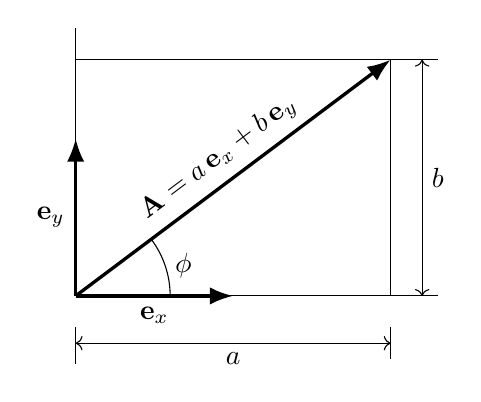
\begin{tikzpicture}[scale=2,
		vector/.style={-{Latex}, very thick}]

    \coordinate (P) at (2, 1.5);

    \draw (0, 0) -- (2.3, 0);
    \draw (0, 0) -- (0, 1.7);

	\draw[vector] (0, 0) -- (P) node [midway, above, rotate=37] {$\vb{A} = a \, \vb{e}_{x} + b \, \vb{e}_{y}$};
    \draw (2, 0) --(P);
    \draw (0, 1.5) -- (P);

    \draw (P) -- (2.3, 1.5);
    \draw [<->] (2.2, 0) -- (2.2, 1.5) node[midway, right] {$b$};
    \draw (0, -0.2) -- (0, -0.43);
    \draw (2, -0.2) -- (2, -0.4);
    \draw [<->] (0, -0.3) -- (2, -0.3) node[midway, below] {$a$};

    \draw[vector] (0, 0) -- (1, 0) node [midway, below] {$\vb{e}_{x}$};
    \draw[vector] (0, 0) -- (0, 1) node [midway, left] {$\vb{e}_{y}$};

    \draw (0.6, 0) arc(0:36.87:0.6) node[midway, right] {$\phi$};
    
\end{tikzpicture}
\end{document}